\documentclass{standalone}
\usepackage{tikz}
\usepackage{ctex,siunitx,bm}
\setCJKmainfont{Noto Serif CJK SC}
\usepackage{tkz-euclide,ninecolors}
\usepackage{amsmath}
\usetikzlibrary{patterns, calc}
\usetikzlibrary {decorations.pathmorphing, decorations.pathreplacing, decorations.shapes,}
\begin{document}
\small
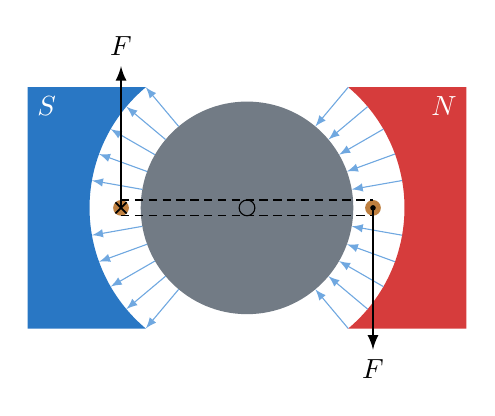
\begin{tikzpicture}[>=latex,yscale=1.0]
  \fill[azure4!15!gray](0,0)circle(1.35);
  \draw(0,0)circle(0.1);
  \fill[brown](-1.6,0)circle(0.1)(1.6,0)circle(0.1);
  \draw[semithick]([shift=(-135:0.1)]-1.6,0)--++(45:0.2)([shift=(135:0.1)]-1.6,0)--++(-45:0.2);
  \fill(1.6,0)circle(1pt);
  \draw[densely dashed](-1.6,0.1)--(1.6,0.1)(-1.6,-0.1)--(1.6,-0.1);
  \fill[azure5](130:2)arc(130:230:2)--++(-1.5,0)--([xshift=-1.5cm]130:2)node[text=white,below right]{$S$}--(130:2);
  \fill[red5](50:2)arc(50:-50:2)--++(1.5,0)--([xshift=1.5cm]50:2)node[text=white,below left]{$N$}--(50:2);
  \foreach \x in {130,140,...,170,190,200,...,230}
  {
    \draw[azure7,->](\x:1.35)--(\x:2.0);
  }
  \foreach \x in {50,40,...,10,-10,-20,...,-50}
  {
    \draw[azure7,->](\x:2.0)--(\x:1.35);
  }
  \draw[thick,->](-1.6,0)--++(0,1.8)node[above]{$F$};
  \draw[thick,->](1.6,0)--++(0,-1.8)node[below]{$F$};
\end{tikzpicture}
\end{document}